\documentclass[10pt]{scrartcl}			%Dokumentenart
\usepackage{polyglossia}					%Sprache
\usepackage{12many}					%Mengen
\usepackage{amsmath}					%Matheumgebung
\usepackage{amsopn}					%Matheoperatoren
\usepackage{amssymb}					%Mathesymbole
\usepackage{amsthm}					%Mathetheorem
\usepackage{array}						%Tabellenumgebung
\usepackage{bbm}						%Mengensymbol
\usepackage[style=numeric]{biblatex}	%Bibliographie
\usepackage{blindtext}					%Blindtext
\usepackage{booktabs}					%Tabellen
\usepackage{braket}						%Dirac-Schreibweise
\usepackage{colortbl}					%Farbe in Tabelle
\usepackage[style=german]{csquotes}	%Anführungszeichen
\usepackage{empheq}					%umrahmte Gleichungen
\usepackage{fancybox}					%Boxen
\usepackage[Bjornstrup]{fncychap}		%Kapitellayout
\usepackage{graphicx}					%Graphik
\usepackage{marvosym}					%Alltagssymbole
\usepackage{listings}					%Codeumgebung
\usepackage{marginnote}				%Randkommentare
\usepackage{mathdots}					%Punkte
\usepackage{mathtools}					%Bugfix ams
\usepackage{microtype}					%Makrotypographie
\usepackage{multirow}					%mehrfache Zeilen
\usepackage{pdfpages}					%Pdf-seiten
\usepackage{pgfplots}					%Diagramme
\usepackage{relsize}						%Größenangaben
\usepackage{scrlayer-scrpage}			%Kopfzeile
\usepackage{siunitx}						%Einheiten
\usepackage{subcaption}					%Gleitumgebung Graphik
\usepackage{tikz}						%Zeichnen
\usepackage{upgreek}					%Griechische Buchstaben
\usepackage{xcolor}						%Farben
\usepackage{xltxtra}						%fontec
\pgfplotsset{compat=1.15}
\setmainlanguage{german}
\setmainfont{Linux Libertine O}

\title{Versuch 80: Szintillatoren}
\subtitle{Python-Code}
\author{Nils Schmitt \and Timo Kleinbek}
\date{}
\usepackage{hyperref}					%Verweise, muss am Ende stehen

\begin{document}
\centering
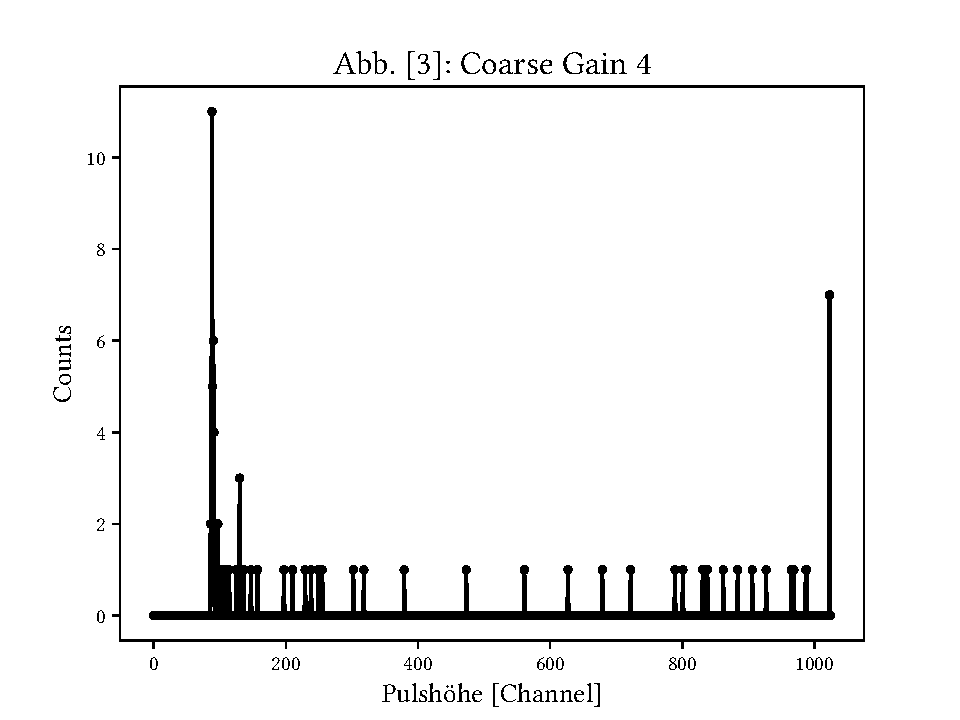
\includepdf[pages=-, landscape=true]{f80_abb_3.pdf}
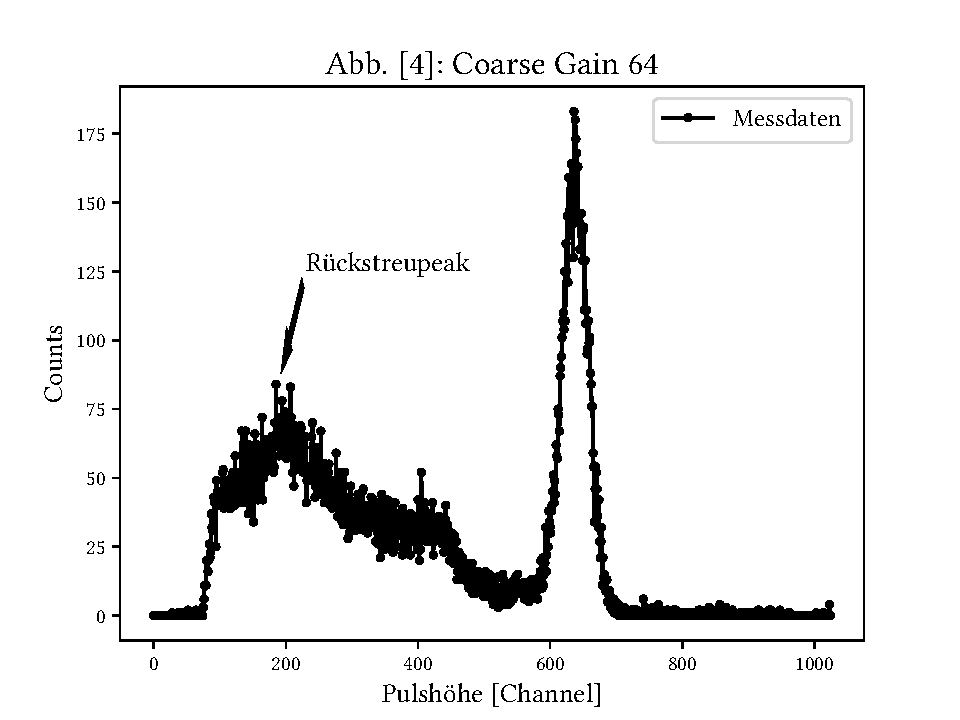
\includepdf[pages=-, landscape=true]{f80_abb_4.pdf}
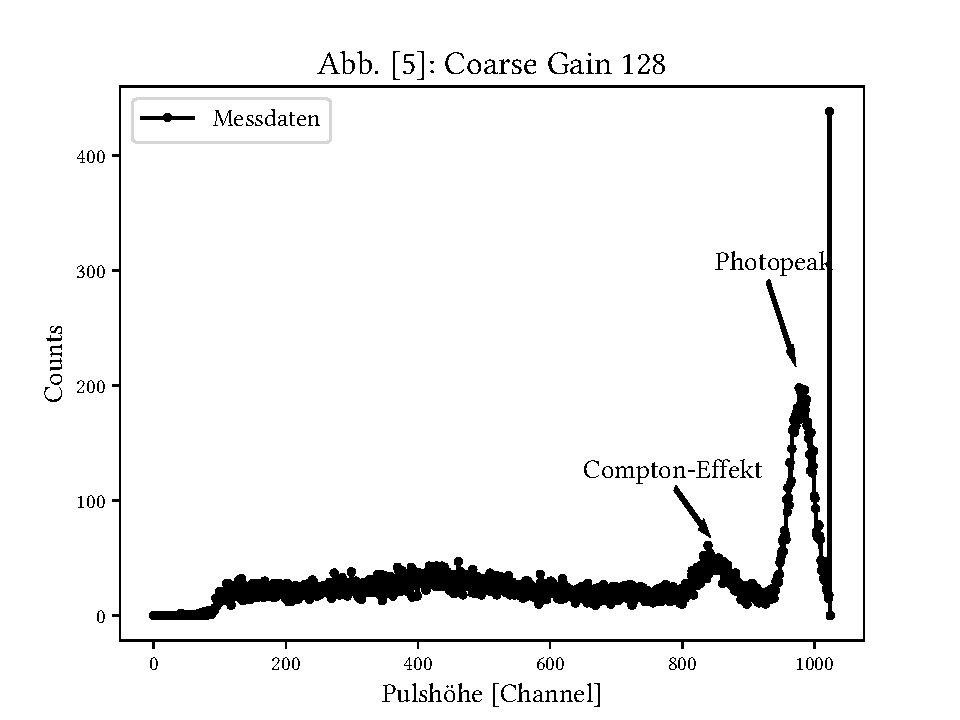
\includepdf[pages=-, landscape=true]{f80_abb_5.pdf}
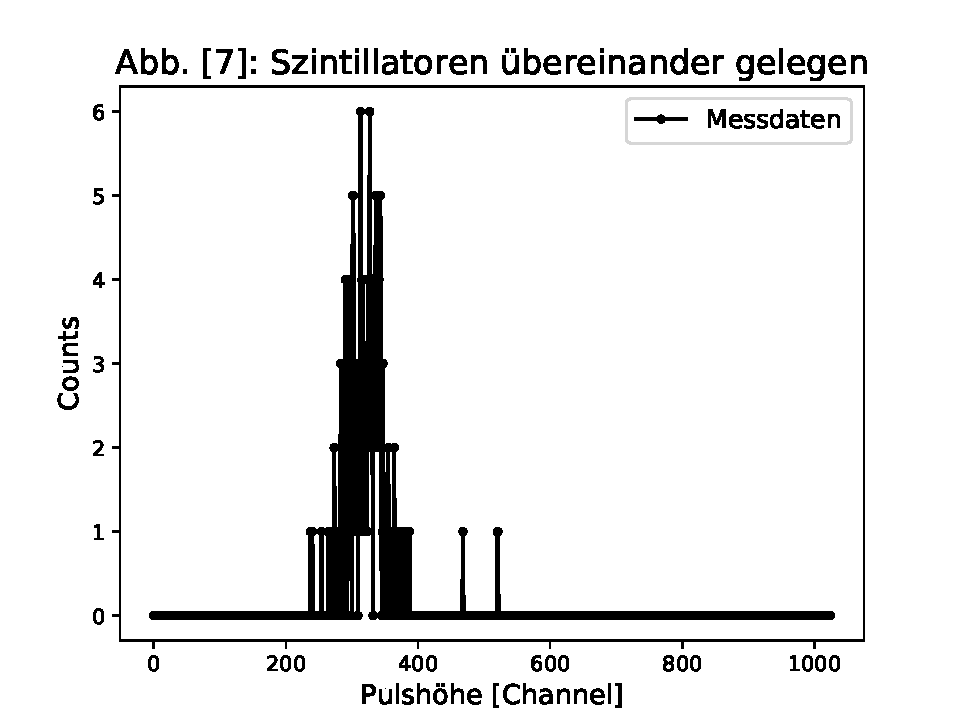
\includepdf[pages=-, landscape=true]{f80_abb_7.pdf}
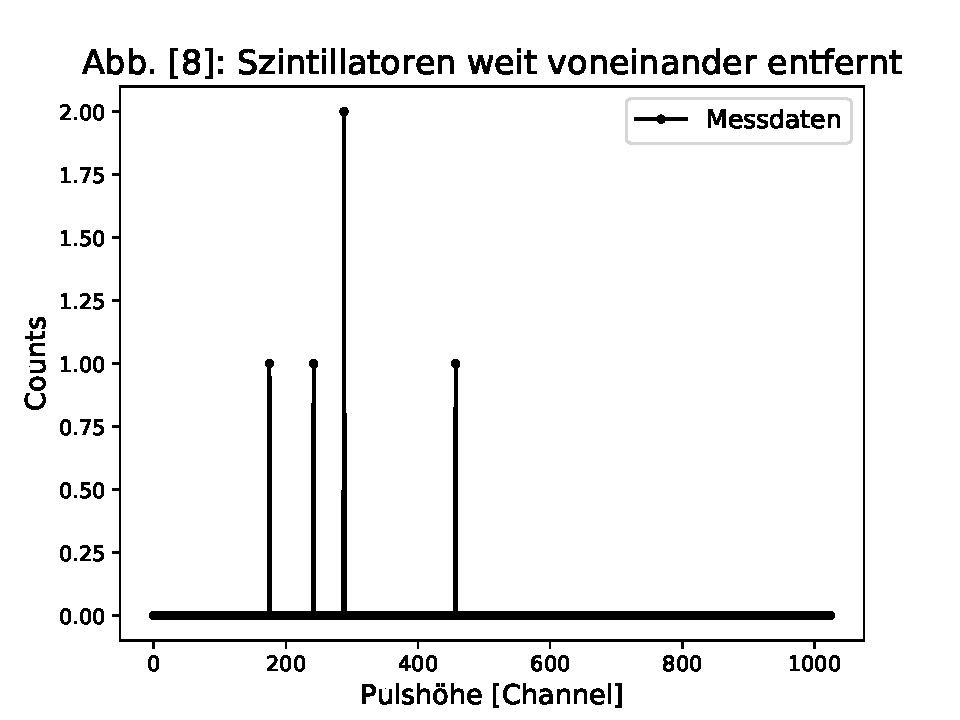
\includepdf[pages=-, landscape=true]{f80_abb_8.pdf}
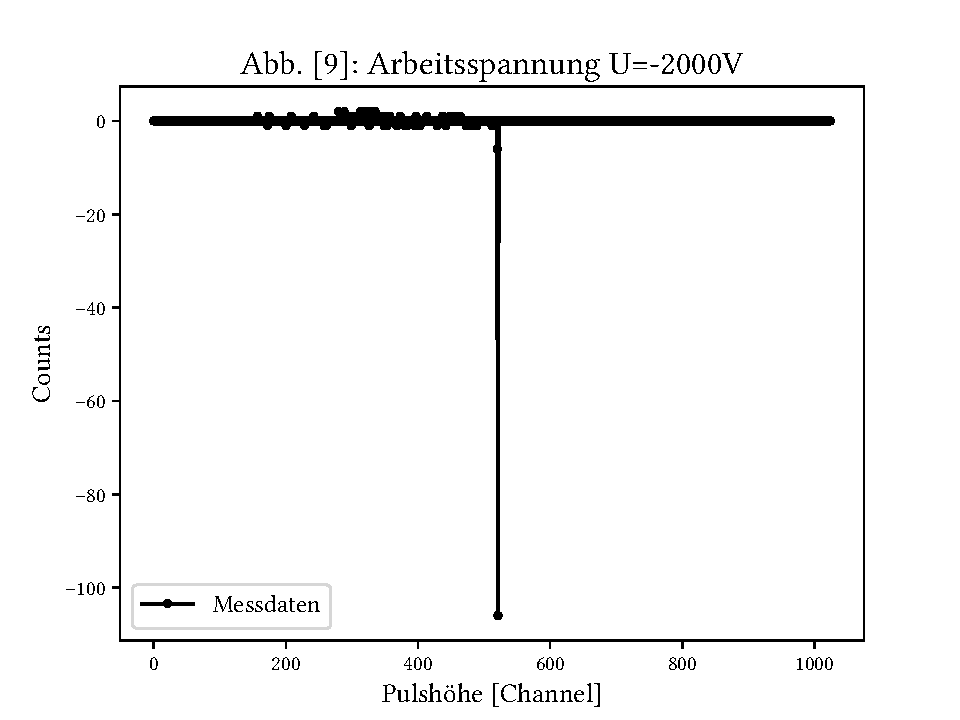
\includepdf[pages=-, landscape=true]{f80_abb_9.pdf}
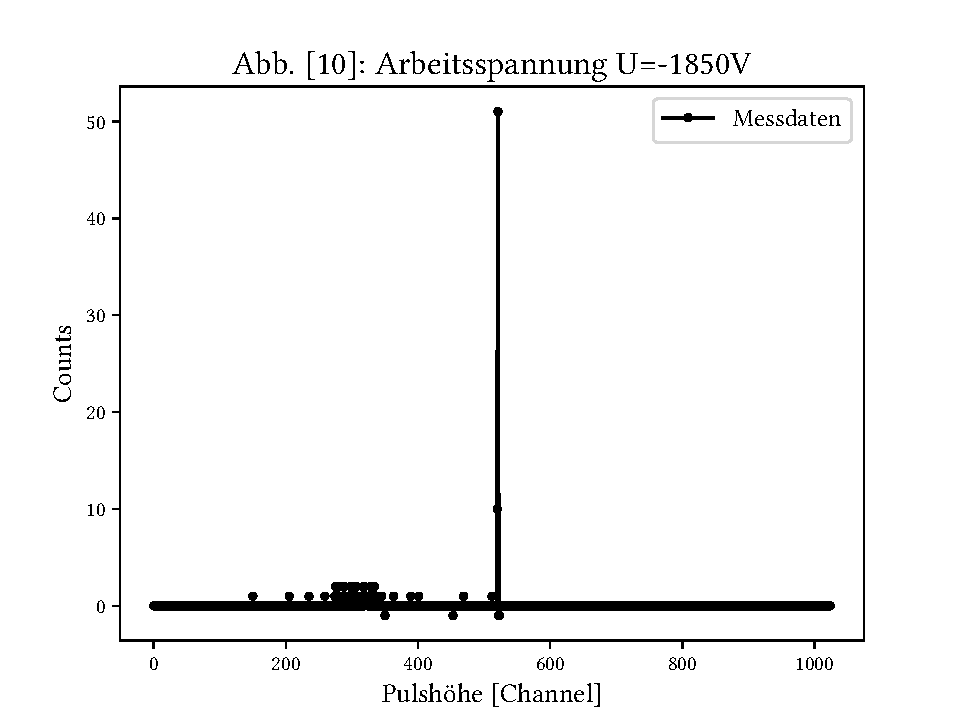
\includepdf[pages=-, landscape=true]{f80_abb_10.pdf}
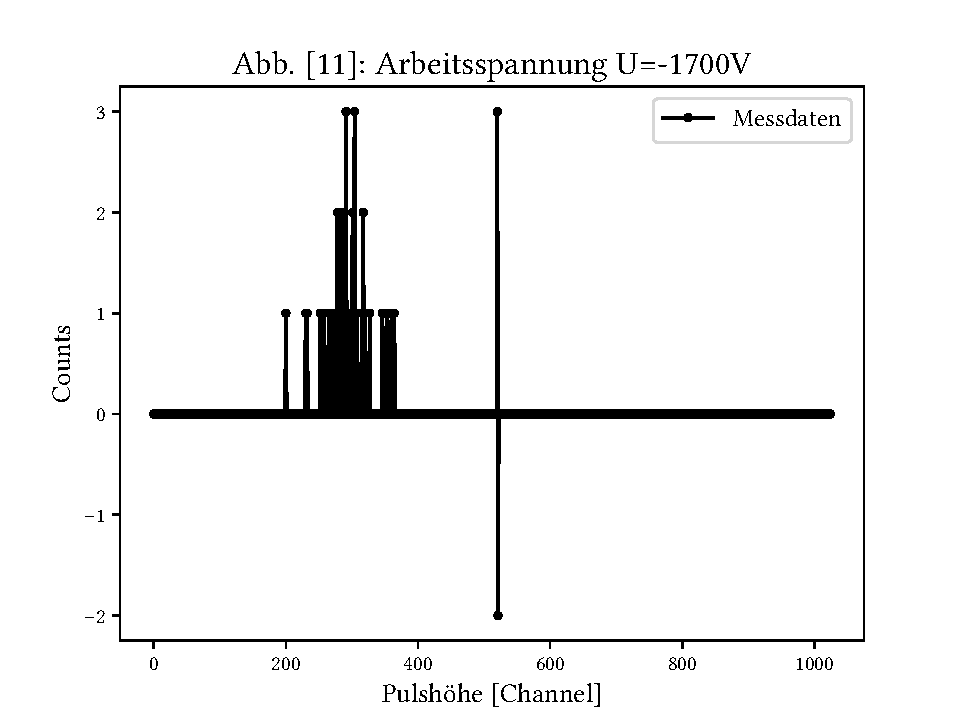
\includepdf[pages=-, landscape=true]{f80_abb_11.pdf}
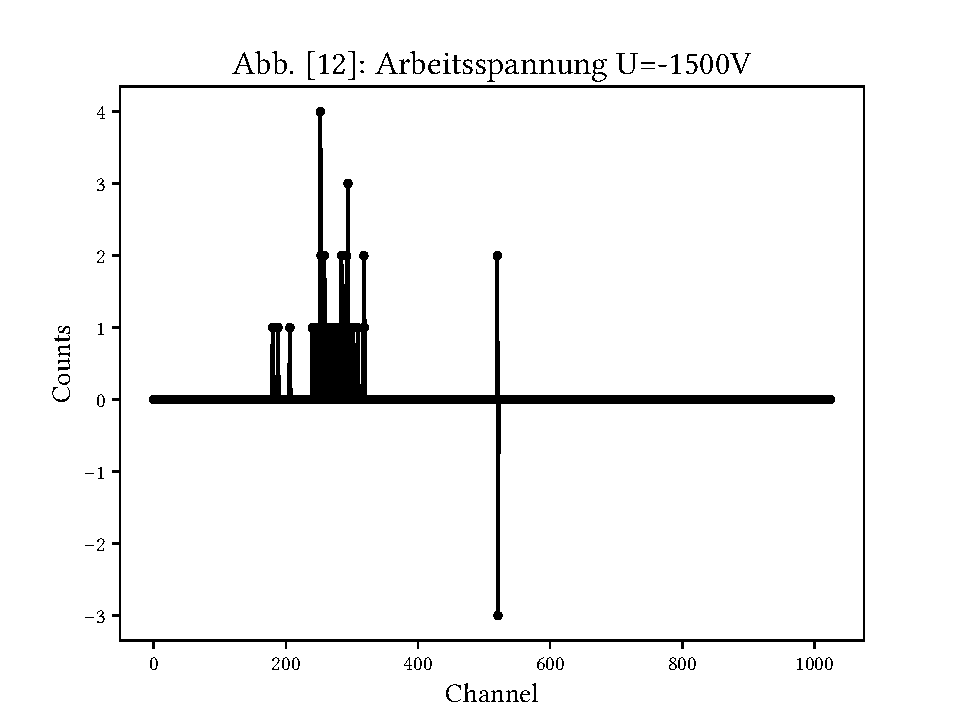
\includepdf[pages=-, landscape=true]{f80_abb_12.pdf}
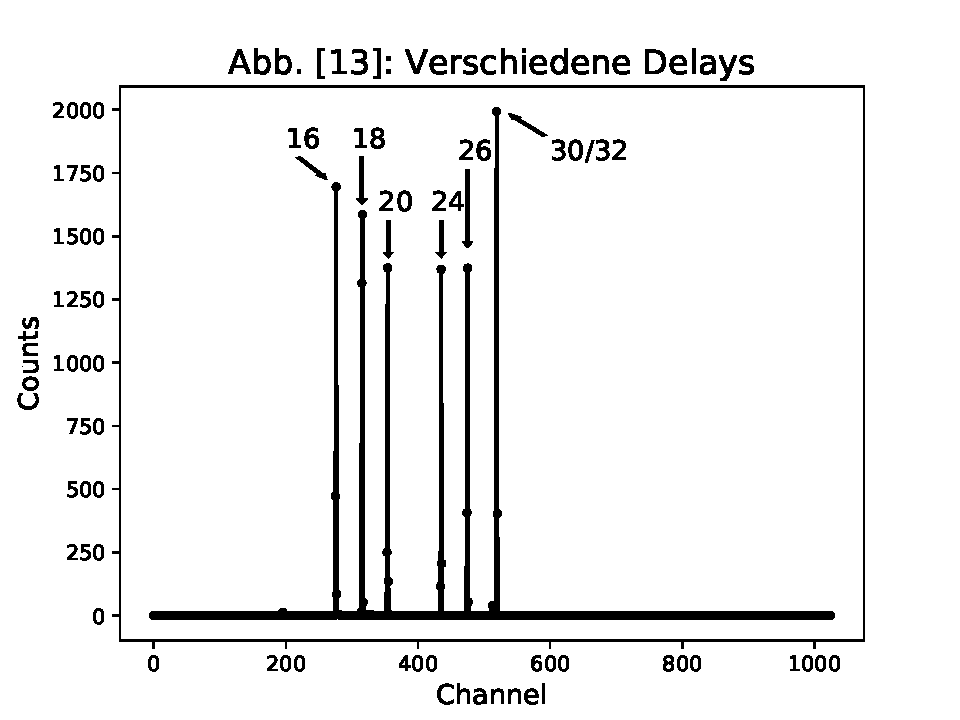
\includepdf[pages=-, landscape=true]{f80_abb_13.pdf}
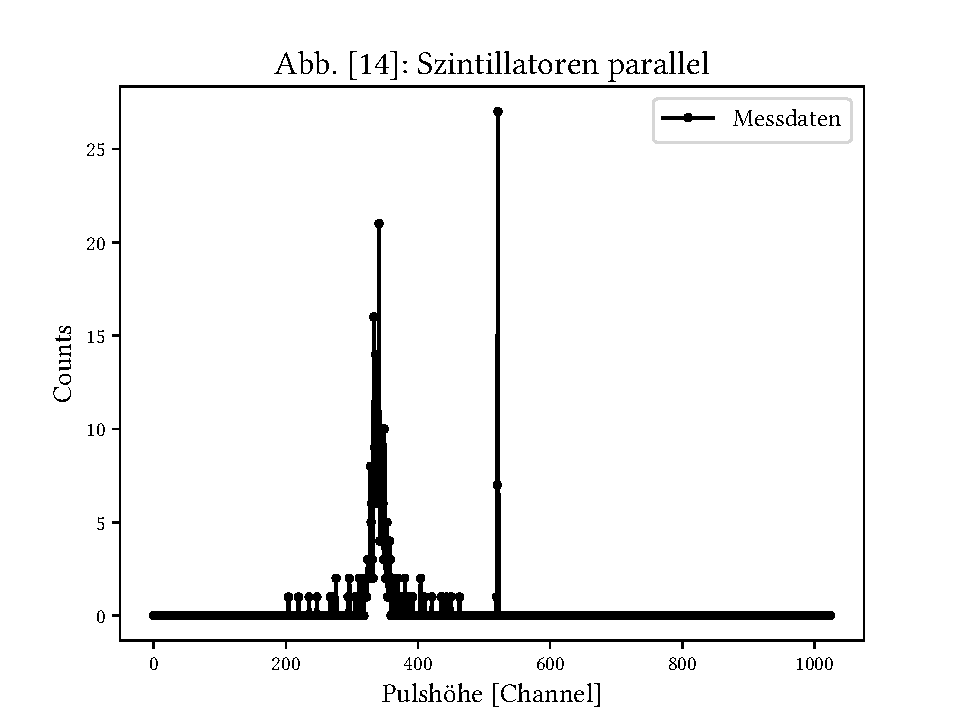
\includepdf[pages=-, landscape=true]{f80_abb_14.pdf}
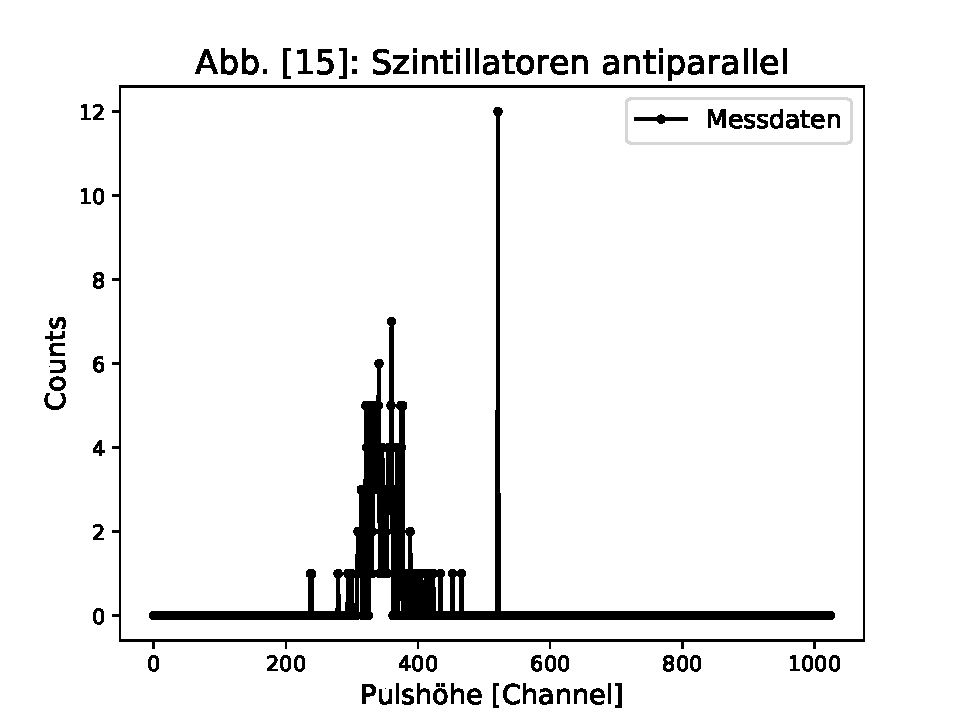
\includepdf[pages=-, landscape=true]{f80_abb_15.pdf}
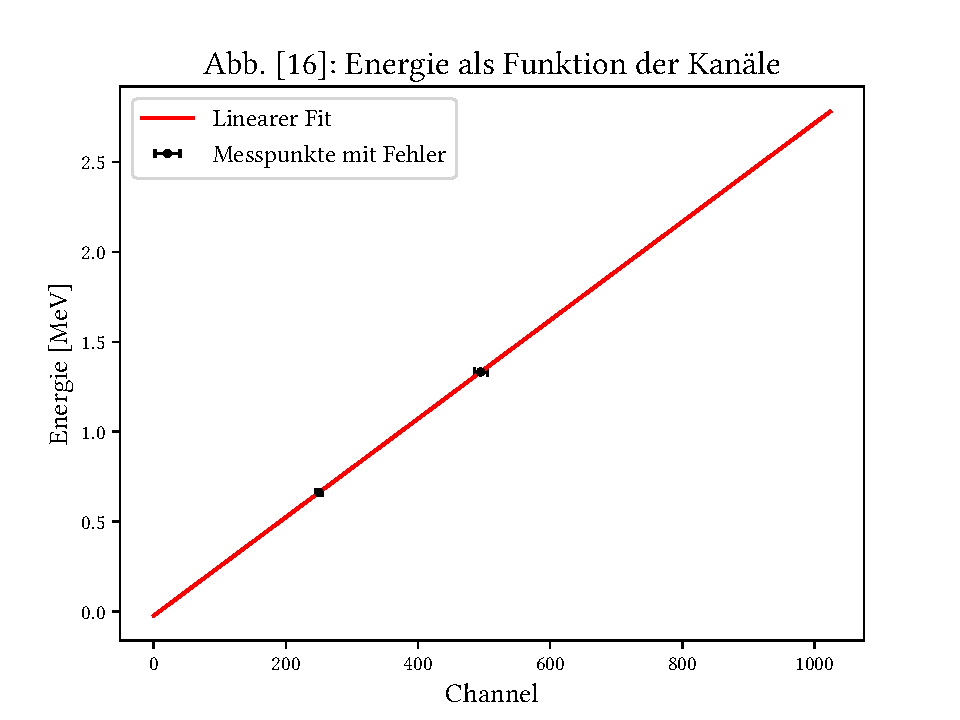
\includepdf[pages=-, landscape=true]{f80_abb_16.pdf}
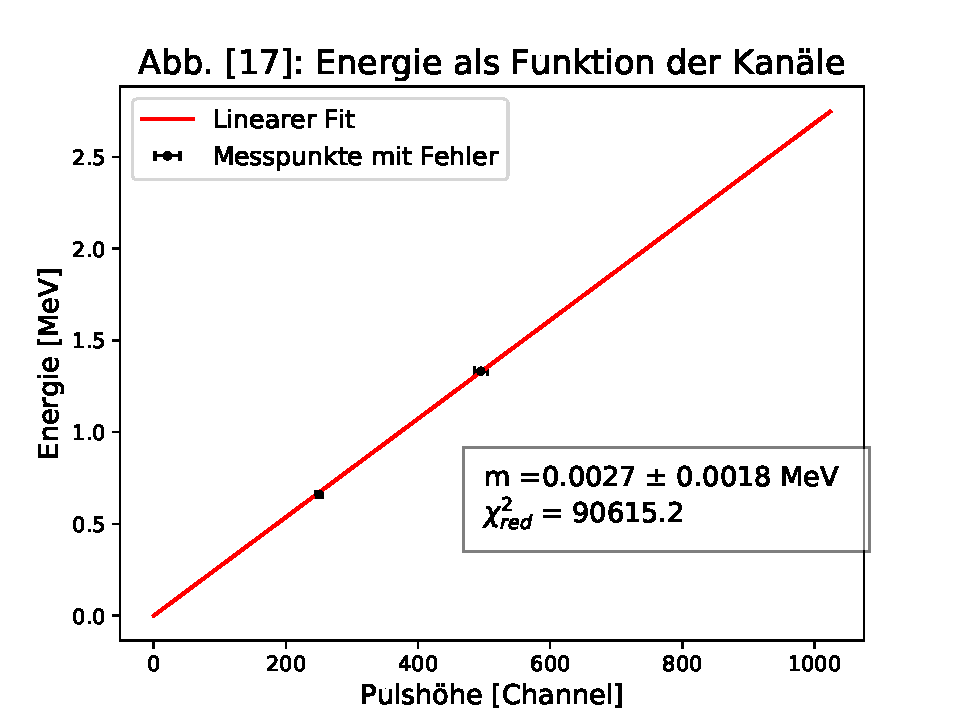
\includepdf[pages=-, landscape=true]{f80_abb_17.pdf}
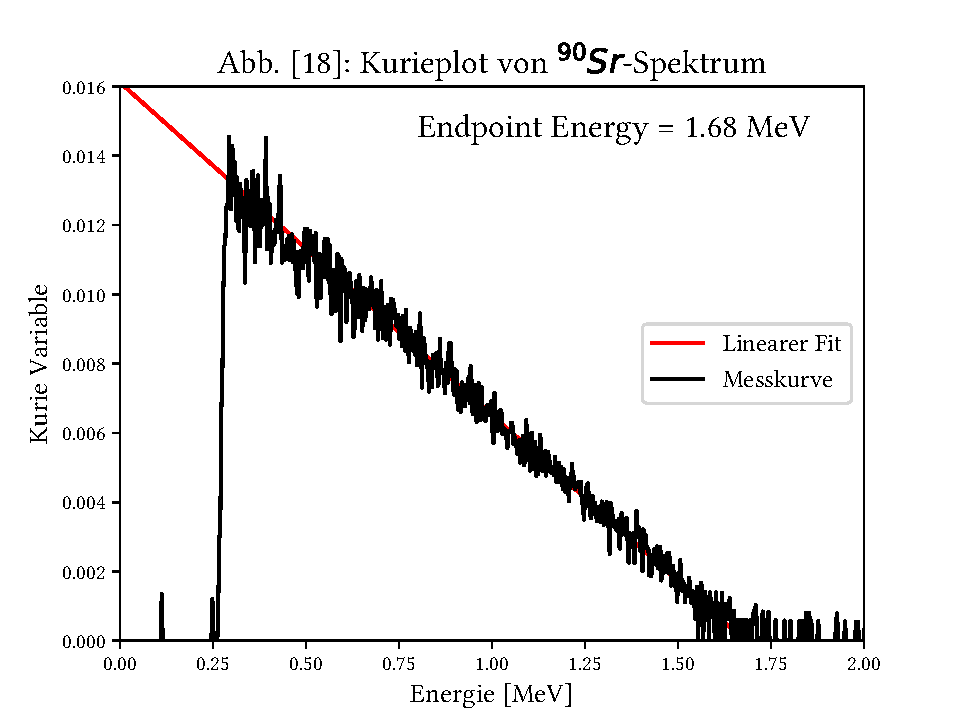
\includepdf[pages=-, landscape=true]{f80_abb_18.pdf}
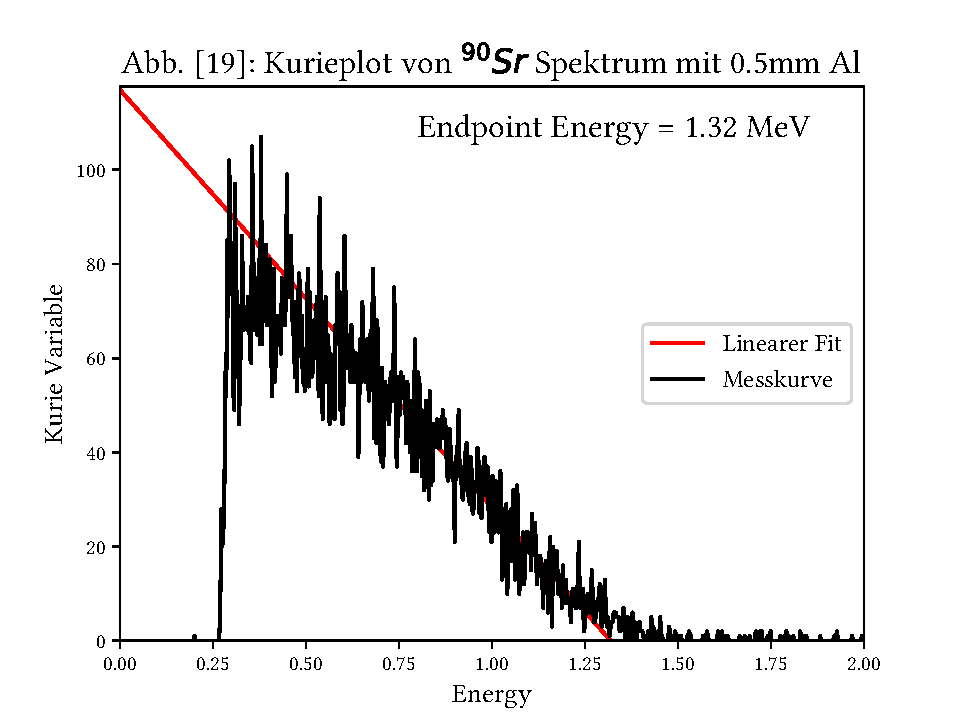
\includepdf[pages=-, landscape=true]{f80_abb_19.pdf}
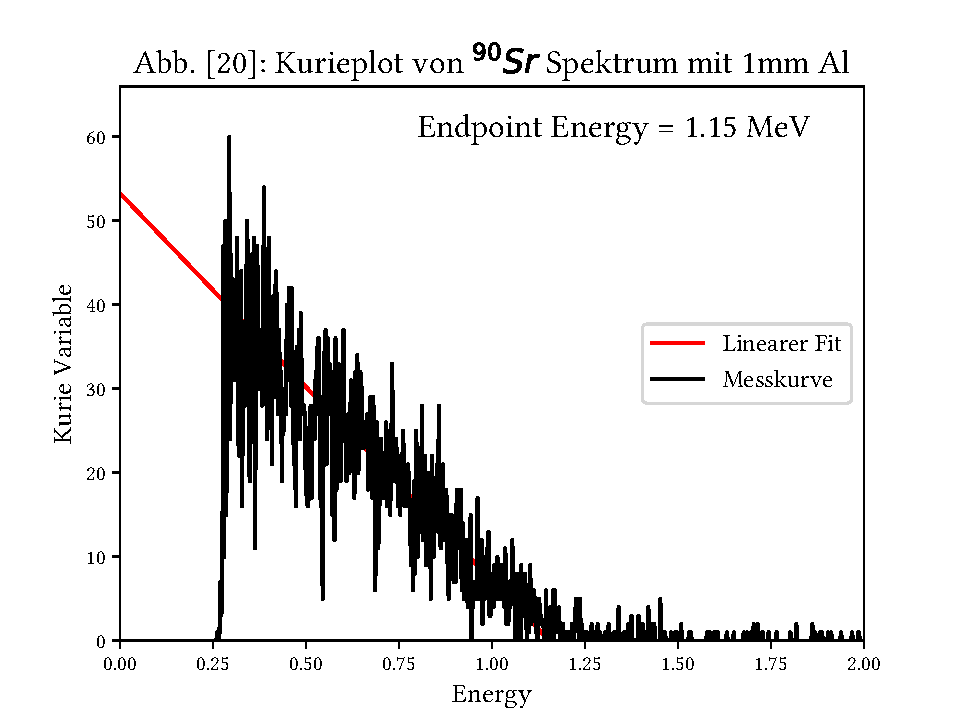
\includepdf[pages=-, landscape=true]{f80_abb_20.pdf}
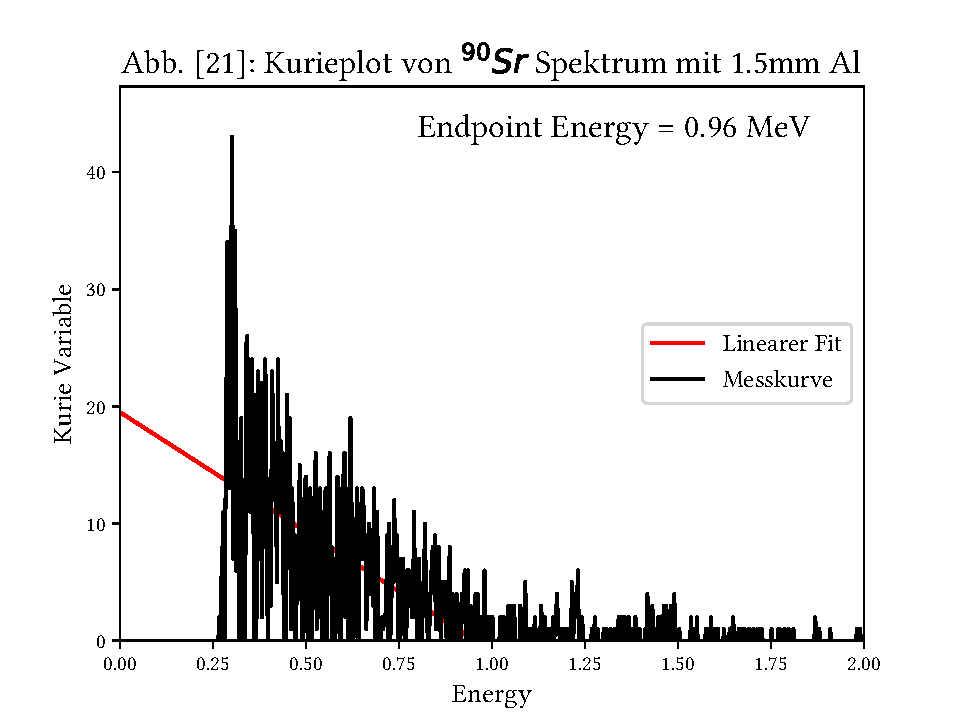
\includepdf[pages=-, landscape=true]{f80_abb_21.pdf}
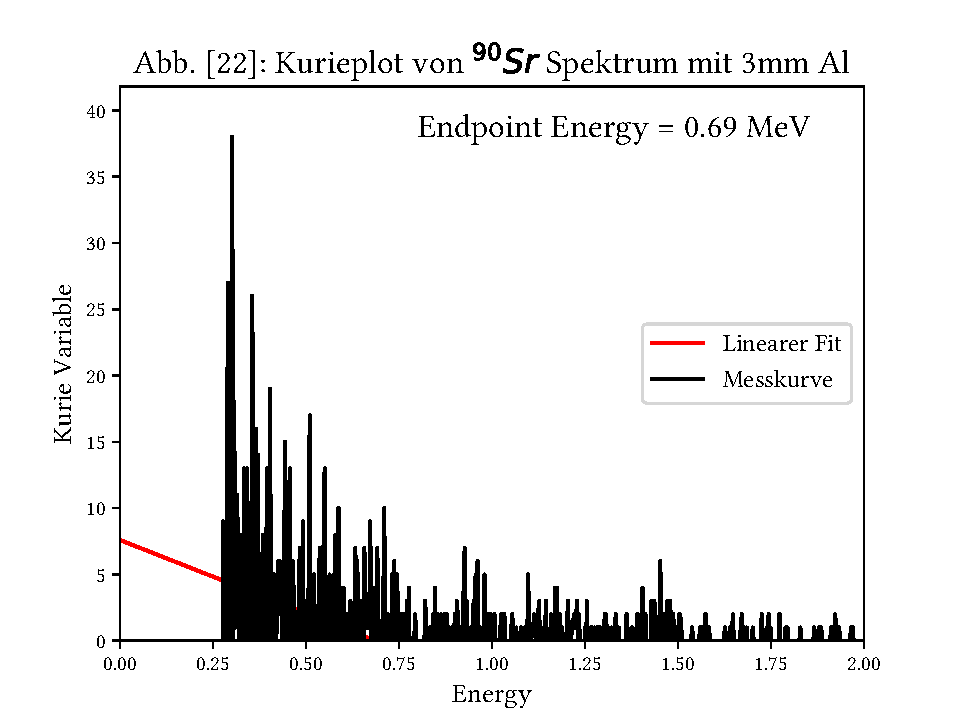
\includepdf[pages=-, landscape=true]{f80_abb_22.pdf}
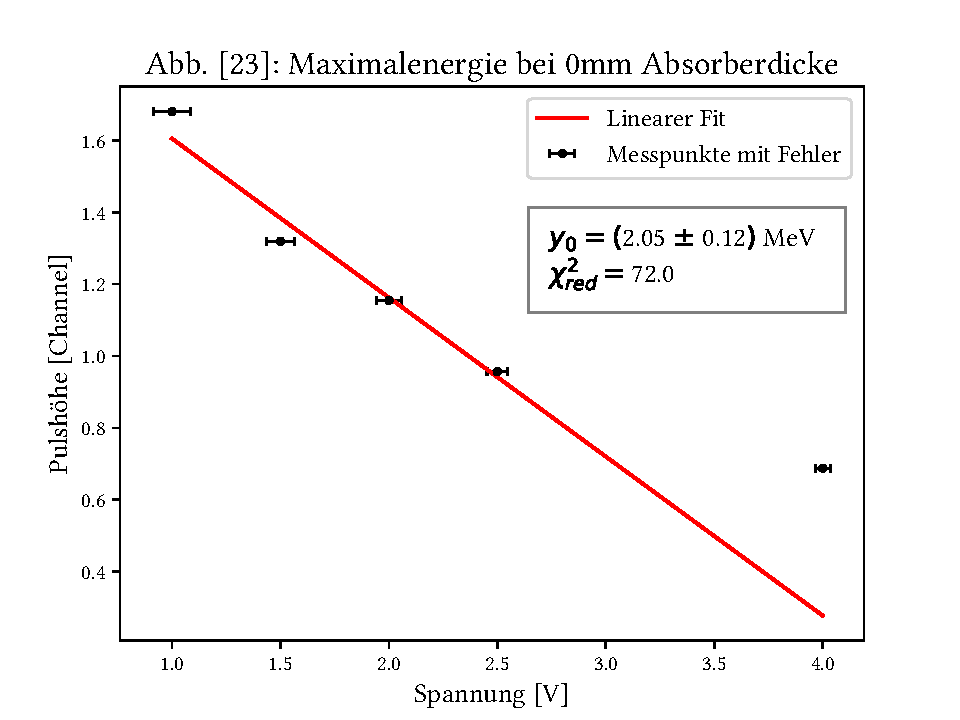
\includepdf[pages=-, landscape=true]{f80_abb_23.pdf}
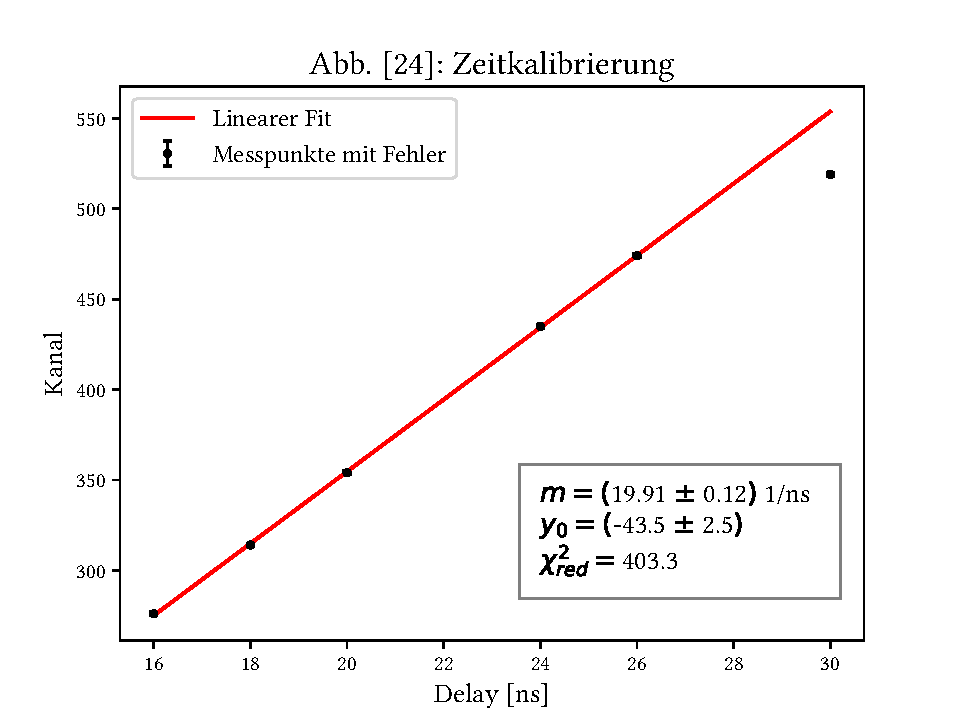
\includepdf[pages=-, landscape=true]{f80_abb_24.pdf}
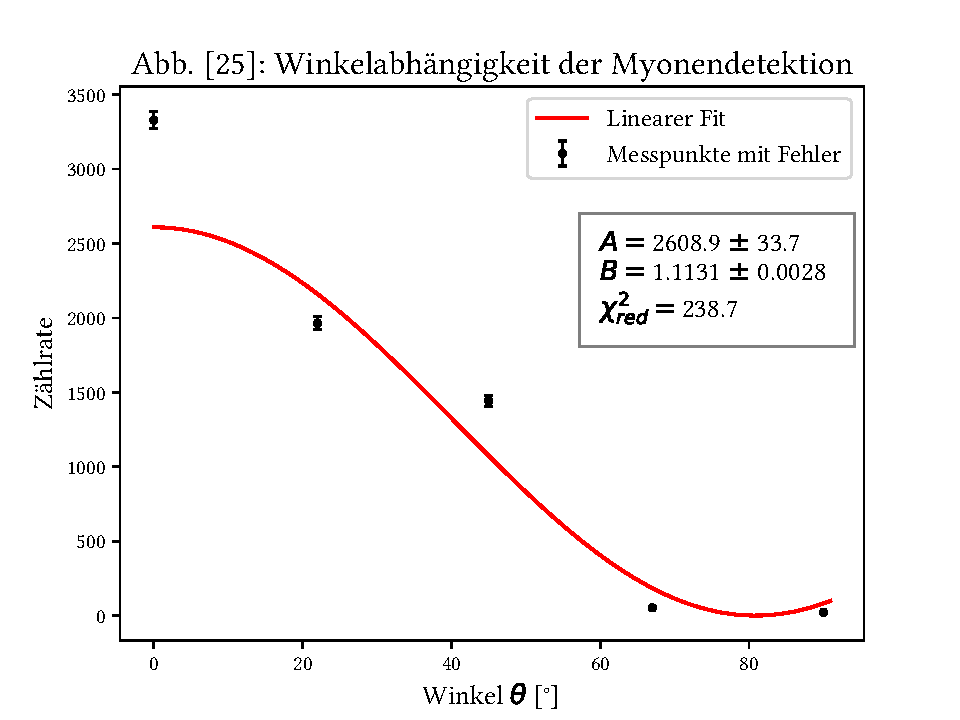
\includepdf[pages=-, landscape=true]{f80_abb_25.pdf}
\end{document}